\documentclass[a4,center]{NAR} %SAM removed fleqn
\usepackage{hyperref} %added by SAM
\usepackage[nodisplayskipstretch]{setspace} %added by SAM 
\setstretch{1.5} %added by SAM
\usepackage{subfig} %added by SAM
\title{Ribofilio manuscript: supplementary document}

\begin{document}
\onecolumn



\begin{figure} [h]
\centering
\begin{tabular}{ll}
 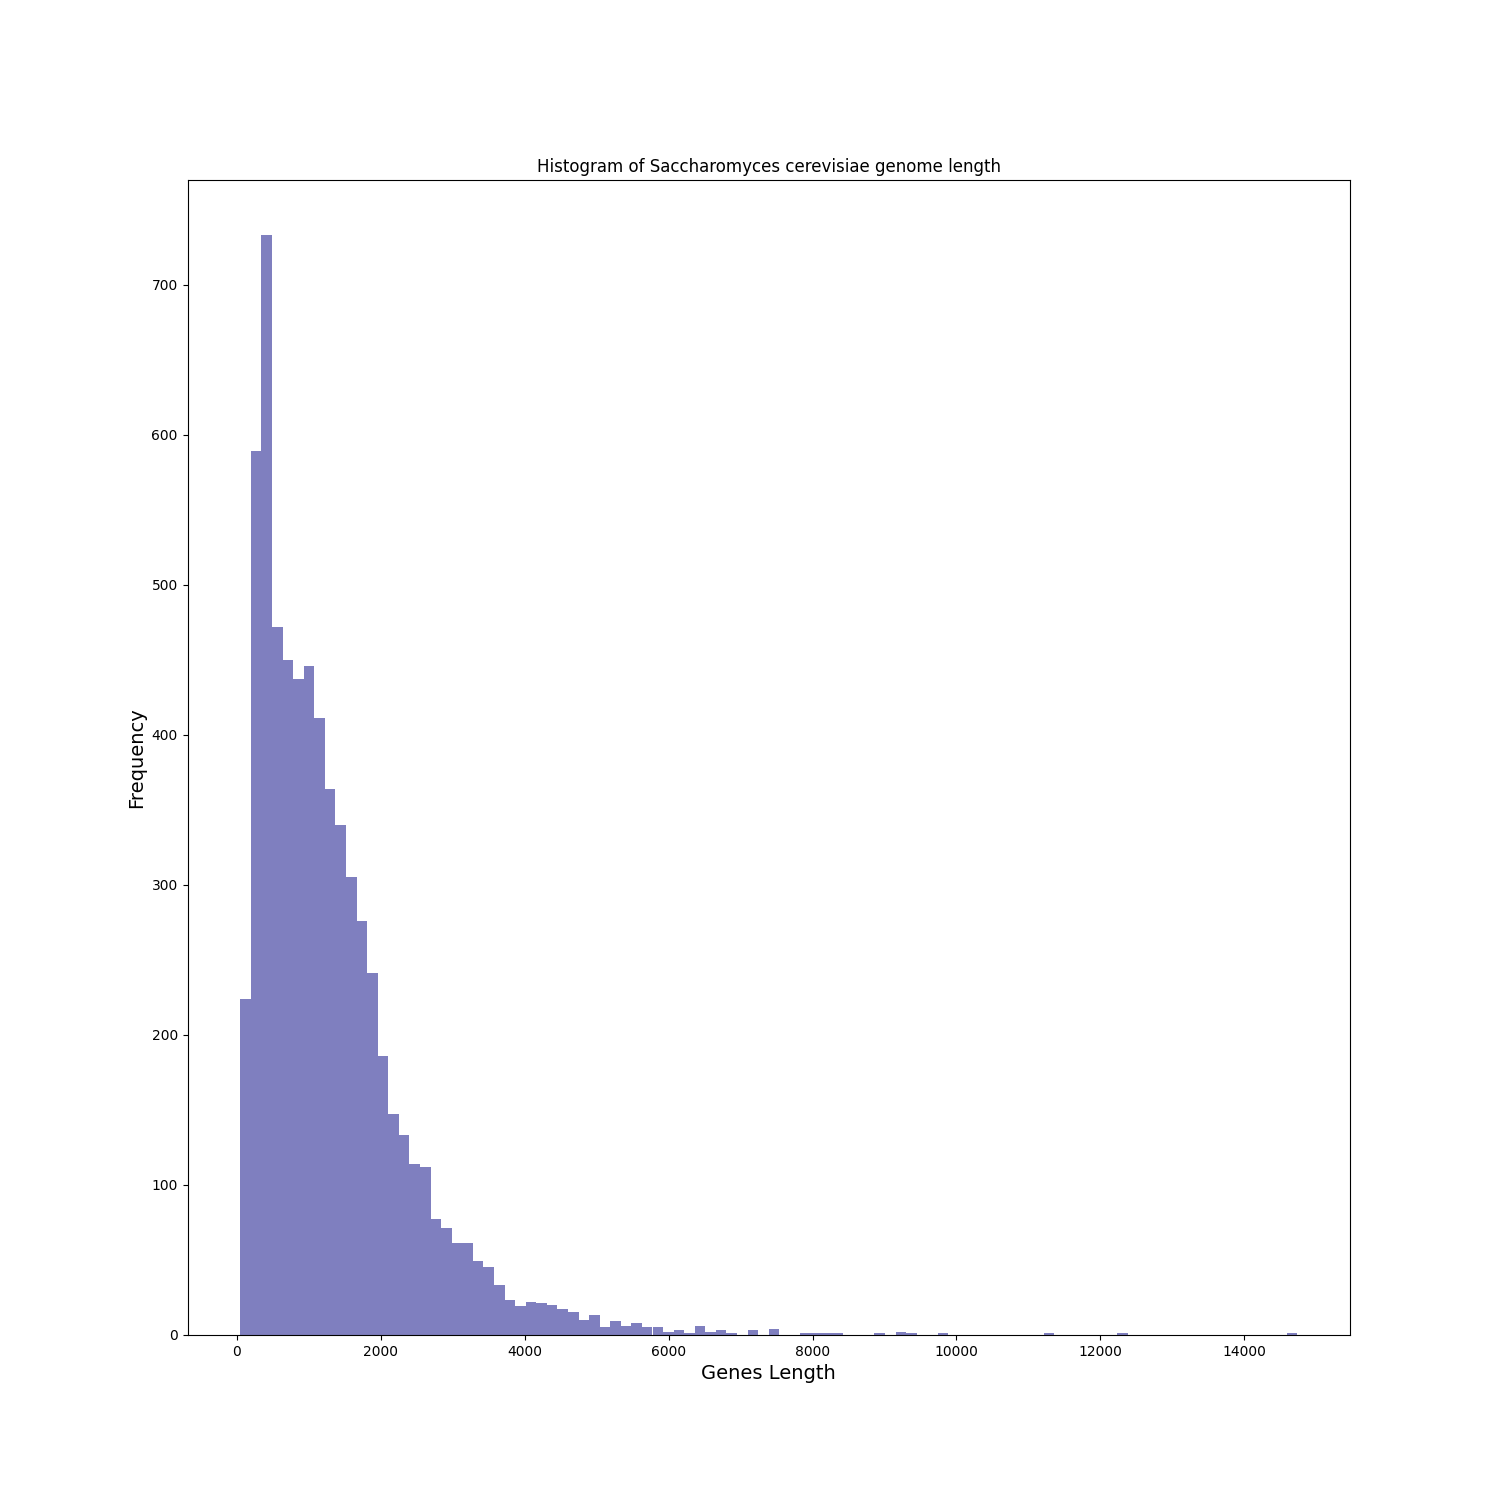
\includegraphics[width=12cm,height=12cm]{yeast.fa.png} \\
 \\[0.1pt]
\end{tabular}
\caption{Saccharomyces cerevisiae Genome Distribution}\label{supp-fig1}
\end{figure}

\clearpage



\begin{table*}[b]
\tableparts{%
\caption{Unique alignments percentages for each dataset. See main text Table 1 for the respective GEO coordinates}
\label{stab1}%
}{%
\begin{tabular} {|l|l|l|}
\hline
Dataset & FP \%& mRNA \%\\
\hline
D1&26.10  &34.21 \\
\hline
D2 &35.43&39.63 \\ 
\hline
D3 &34.26&32.21\\
\hline
D4 &24.21 &33.88\\
\hline
D5 &27.21 &41.13\\
\hline
D6 &35.40&34.75\\
\hline
D7 &70.12&38.13\\
\hline
D8 &37.04&37.68\\
\hline
D9 &62.33&35.29\\
\hline
D10 &46.64&28.04\\
\hline
\end{tabular}%
}

\end{table*}


\begin{table*}[b]
\tableparts{%
\caption{Adapters trimmed used for each dataset as confirmed by authors. See main text Table 1 for the respective GEO coordinates}
\label{stab1}%
}{%
\begin{tabular}{|l|l|}
\hline
Adapter & Datasets\\
\hline
CTGTAGGCACCATCAAT&D1, D2, D3, D4, D5, D6 \\
\hline
PolyA & D7, D8, D9, D10 \\ 
\hline
\end{tabular}%
}

\end{table*}



\begin{table*}[b]
\tableparts{%
\caption{Significance test of D1 vs D4, D2 vs D5, and D3 vs D6. Column1: Dataset ID. (See main text Table 1 for the respective GEO coordinates). Column 2: Pvalue}
\label{stab1}%
}{%
\begin{tabular} {|l|l|}
\hline
Dataset & Pvalue\\
\hline
D1 vs D4 &0.0001 \\
\hline
D2 vs D5 &\textless 0.00001 \\ 
\hline
D3 vs D6&0.0001\\
\hline
\end{tabular}%
}

\end{table*}


\begin{table*}[b]
\tableparts{%
\caption{Significance test of D7 vs D9 and D8 vs D10  Column1: Dataset ID. (See main text Table 1 for the respective GEO coordinates). Column 2: Pvalue}
\label{stab2}%
}{%
\begin{tabular} {|l|l|}
\hline
Dataset & Pvalue\\
\hline
D7 vs D9 &0.2602   \\
\hline
D8 vs D10 &0.2338 \\ 
\hline
\end{tabular}%
}

\end{table*}


%===========================================
%Gene Ontology ID description 
%===========================================
\begin{table}[h]
\tableparts{%
\caption{Gene Ontology Description. Column 1 is Gene Ontology ID. Column 2 is Gene Ontology Description. Column 3 is set size.}
\label{stab3}%
}{%
\begin{tabular}{|l|l|l|}
\toprule
Gene Ontology ID &Gene Ontology Description & Set Size
\\
\hline
GO:0000462&Maturation of SSU-rRNA from tricistronic rRNA transcript & 70\\
\hline
GO:0000466&Maturation of 5.8S rRNA from tricistronic rRNA transcript & 15\\
\hline
GO:0002181& Cytoplasmic Translation &151\\
\hline
GO:0003723& RNA binding &315\\
\hline
GO:0005840& Ribosome &171\\
\hline
GO:0006364& rRNA processing &111\\
\hline
GO:0006396& RNA processing &31\\
\hline
GO:0006406& mRNA Export from Nucleus &36\\
\hline
GO:0006412& Translation &186 \\
\hline
GO:0006950& Response to Stress &33\\
\hline
GO:0007049& Cell Cycle &91\\
\hline
GO:0009651& Response to Salt Stress &20 \\
\hline
GO:0015934& Large Ribosomal Subunit &18\\
\hline
GO:0016458& Gene Silencing &2
\\
\hline
GO:0022625& Cytosolic Large Ribosomal Subunit &83\\
\hline
GO:0022626& Cytosolic Ribosome &12 \\
\hline 
GO:0022627& Cytosolic Small Ribosomal Subunit &66\\
\hline
GO:0022857& Transmembrane Transporter Activity &111\\
\hline
GO:0030490& Maturation of SSU-rRNA &15\\
\hline
GO:0030687& Preribosome, Large Subunit Precursor &52\\
\hline
GO:0042254& Ribosome Biogenesis &64\\
\hline
GO:0042274& Ribosomal Small Subunit Biogenesis &30\\
\hline
GO:0042255& Ribosome Assembly &4\\
\hline
GO:0003735 &Structural Constituent of Ribosome&220\\
\hline
GO:0003743 &Translation Initiation Factor activity &37\\
\hline
GO:0030684&Preribosome&2\\
\hline
GO:0044249&Cellular biosynthetic process&6\\
\hline
GO:0006457&Protein folding&85\\
\hline
GO:0030686&90S Preribosome&22\\
\hline
GO:0008135&Translation factor activity, RNA binding&1\\
\hline
GO:0030529&Ribonucleoprotein complex&6\\
\hline
GO:0015935&Small Ribosomal subunit
&18\\
\hline
\end{tabular}%
}
 
\end{table}

\begin{table*}[t]
\tableparts{%
\caption{Drop-off rate per codon for dataset D1 per GO subsets: Column 1: GO ID  (see Supplementary Table 01 for the respective GO names). Column 2: Drop-off rate (R). Column 3: Drop-off rate per codon (r). Column 4: RMSE. Column 6: R square Column 7: Standard Error Estimate (SE).Column 8: Confidence Interval 95\%. Column 9: Pvalue: Null Hypothesis that the drop-off rate is not different from a slope of zero}
\label{stab4}%
}{%
\begin{tabular} {|l|l|l|l|l|l|l|l|}
\hline
\multicolumn{7}{|c|}{D1} \\
\hline
GO&Drop-off (R) & Dropoff per codon (r)&RMSE& Rsquare&SE&CI &Pvalue\\
\hline
GO:0000462&-0.0136&-0.0008&0.1568&0.301&0.0016&R$\pm$0.0031&\textless 0.00001\\
\hline
GO:0000466&-0.0114&-0.0007&0.447&0.137&0.0039&R$\pm$0.0076&0.0019\\
\hline
GO:0002181&-0.0139&-0.0008&0.4688&0.1139&0.0057&R$\pm$0.0113&0.0082\\
\hline
GO:0003723&-0.0142&-0.0008&0.1771&0.2837&0.0052&R$\pm$0.0102&0.0034\\
\hline
GO:0005840&0.0023&0.0001&0.1523&0.0037&0.0041&R$\pm$0.0081&0.2852\\
\hline
GO:0006364&-0.0033&-0.0002&0.426&0.051&.0013&R$\pm$0.0026&0.0077\\
\hline
GO:0006396&0.0025&0.0002&0.2275&0.0137&0.0015&R$\pm$0.0029&0.0448\\
\hline
GO:0006406&-0.0153&-0.0009&0.2653&0.2429&0.0049&R$\pm$0.0098&0.0012 \\
\hline
GO:0006412&-0.029&-0.0017&0.4762&0.2228&0.01&R$\pm$0.0198&0.0023\\
\hline
GO:0007049&-0.0193&-0.0011&0.2507&0.378&0.0046&R$\pm$0.0092  &\textless 0.00001\\
\hline
GO:0009651&-0.0191&-0.0011&0.1238&0.4797&0.0026   &R$\pm$0.0052&\textless 0.00001\\
\hline
GO:0015934&-0.04&-0.0024&3.1911&0.238&0.0115  &R$\pm$0.0228&0.0004\\
\hline
GO:0016458&-0.0352&-0.0021&1.4971&0.3414&0.0056  &R$\pm$0.0111&\textless 0.00001\\
\hline
GO:0022625&-0.0359&-0.0021&0.0879&0.3203&0.0059  &R$\pm$0.012&\textless 0.00001\\
\hline
GO:0022626&-0.0077&-0.0005&0.1348&0.4062&0.0008  &R$\pm$0.0016&\textless 0.00001\\
\hline
GO:0022627&0.0021&0.0001&0.1957&0.0026&0.0038 &R$\pm$0.0075&0.2915\\
\hline
GO:0030490&0.0031&0.0002&0.2414&0.0223&0.002   &R$\pm$0.0041&0.0671\\
\hline
GO:0030687&-0.0327&-0.0019&0.1473&0.5615&0.0032  &R$\pm$0.0064&\textless 0.00001\\
\hline
GO:0042254&-0.0122&-0.0007&0.3784&0.2818&0.0025  &R$\pm$0.005&\textless 0.00001\\
\hline
GO:0042274&-0.014&-0.0008&0.2632&0.187&0.0065  &R$\pm$0.013&0.0171\\
\hline
GO:0042255&-0.0048& -0.0003& 0.2121 & 0.0371 & 0.0031 & R$\pm$0.0062  &0.0638   \\
\hline
GO:0003735 & -0.0465 &-0.0027& 0.1409 & 0.3187 & 0.03  &  R$\pm$0.0609  &  0.0653 \\
\hline
GO:0003743 &-0.0079 &-0.0005& 0.0632 & 0.1874 & 0.0018  &R$\pm$0.0036 & \textless 0.00001  \\
\hline
GO:0006457& -0.0143& -0.0008& 0.0765 & 0.2795&  0.0035&  R$\pm$0.007& 0.0001\\
\hline
GO:0008135&-0.0728 &-0.0042& 0.6495&0.2302 & 0.0305 & R$\pm$0.0639  &  0.0139 \\
\hline
GO:0030529&-0.0501& -0.0029 &1.0464&  0.1873 & 0.0277 & R$\pm$0.0561  & 0.0394   \\
\hline
GO:0030684&-0.0406&-0.0024&0.0796&0.5521&0.0068&R$\pm$0.0141& \textless 0.00001  \\
\hline
GO:0044249&-0.0481& -0.0028 &0.0946 & 0.5671  &0.0093 & R$\pm$0.019 & \textless 0.00001  \\
\hline
GO:0030686&-0.0152& -0.0009& 0.4494&0.3564 & 0.0022&R$\pm$0.0043 &  \textless 0.00001  \\
\hline
GO:0015935&-0.0391&-0.0023&3.4594&0.2245&0.0116  &R$\pm$0.023&0.0005  \\
\hline
GO:0009651&-0.0191 &-0.0011 &0.1238  &0.4797&  0.0026&  R$\pm$0.0052 &    \textless 0.00001 \\
\hline
\end{tabular}%
}

\end{table*}


\begin{table*}[h]
\tableparts{%
\caption{Drop-off rate per codon for dataset D2 per GO subsets: Column 1: GO ID  (see Supplementary Table 01 for the respective GO names). Column 2: Drop-off rate (R). Column 3: Drop-off rate per codon (r). Column 4: RMSE. Column 6: R square Column 7: Standard Error Estimate (SE).Column 8: Confidence Interval 95\%. Column 9: Pvalue: Null Hypothesis that the drop-off rate is not different from a slope of zero}
\label{stab5}%
}{%
\begin{tabular} {|l|l|l|l|l|l|l|l|}
\hline
GO&Drop-off (R) & Dropoff per codon (r)&RMSE&R Square& SE&CI &Pvalue\\
\hline
GO:0000462&0.0028 & 0.0002 & 0.0607 & 0.046 &  0.001  &R$\pm$0.0019 & 0.0021  \\
\hline
GO:0000466&0.0038 & 0.0002  &0.0962&  0.0764  &0.0013 &R$\pm$0.0026 &0.0019 \\
\hline
GO:0002181&0.0081 &0.0005 & 0.1481 & 0.1224&  0.003 &R$\pm$0.006 &0.0044 \\
\hline
GO:0003723&-0.0014 &-0.0001 &0.0317 & 0.0221 & 0.001&R$\pm$0.002& 0.0775 \\
\hline
GO:0005840& 0.0164&  0.001 &  0.0452 & 0.3839&0.0031&R$\pm$0.0063&\textless 0.00001\\
\hline
GO:0006364&0.0055&0.0003&0.0899&0.4201&0.0006&R$\pm$0.0011&\textless 0.00001 \\
\hline
GO:0006396&0.0155&0.0009&0.1116&0.5148&0.0013&R$\pm$0.0026&\textless 0.00001 \\
\hline
GO:0006406&-0.0&-0.0&0.0205&0.0&0.001&R$\pm$0.002&0.4903 \\
\hline
GO:0006412&-0.0033&-0.0002&0.0488&0.0345&0.0019&R$\pm$0.0037&0.0426 \\
\hline
GO:0007049&-0.0081&-0.0005&0.1221&0.1791&0.0026&R$\pm$0.0052&0.0012 \\
\hline
GO:0015934&-0.0081& -0.0005 &0.1808 & 0.1828  &0.0018 & R$\pm$0.0036 &   \textless 0.00001 \\
\hline
GO:0016458&-0.0206 &-0.0012 &0.1388 & 0.6568 & 0.0015 &R$\pm$0.003&\textless 0.00001 \\
\hline
GO:0022625&-0.0005&-0.0&0.0164&0.0004&0.0041&R$\pm$0.0084&0.456 \\
\hline
GO:0022626&-0.0004& -0.0&0.121&0.002&0.0008&R$\pm$0.0016&0.3173 \\
\hline
GO:0022627&0.0212&0.0013&0.0918&0.3647&0.0034&R$\pm$0.0068&\textless 0.00001 \\
\hline
GO:0030490&0.0124&0.0007&0.1628&0.3527&0.0019&R$\pm$0.0037&\textless 0.00001  \\
\hline
GO:0030686&-0.0014&-0.0001&0.1674&0.0133&0.0008&R$\pm$0.0017&0.0441 \\
\hline
GO:0030687&-0.0135&-0.0008&0.0524&0.3805&0.0018&R$\pm$0.0036&\textless 0.00001  \\
\hline
GO:0042254&-0.0008&-0.0&0.1234&0.0052&0.0011&R$\pm$0.0022&0.2347 \\
\hline
GO:0042274&0.0007&0.0&0.0711&0.0022&0.0024&R$\pm$0.0047&0.3825 \\
\hline
GO:0042255&0.0022&0.0001&0.225&0.008&0.0032&R$\pm$0.0065&0.2459\\
\hline
GO:0003735&-0.0146&-0.0009&0.0204&0.2405&0.0073&R$\pm$0.0148&0.0269  \\
\hline
GO:0003743&0.004&0.0002&0.0306&0.109&0.0017&R$\pm$0.0034&0.0103   \\
\hline
GO:0006457&0.0042&0.0003&0.0803&0.0311&0.0076&R$\pm$0.0152&0.2918  \\
\hline
GO:0008135&-0.0471&-0.0028&0.2536&0.2428&0.0191&R$\pm$0.0399&0.0116  \\
\hline
GO:0030529&-0.0121&-0.0007&0.2336&0.0566&0.0114&R$\pm$0.0232&0.149 \\
\hline
GO:0022857&-0.0123&-0.0007&0.0241&0.4399&0.0025&R$\pm$0.005&\textless 0.00001\\
\hline
GO:0030684&-0.0272&-0.0016&0.0431&0.5057&0.005&R$\pm$0.0103&\textless 0.00001\\
\hline
GO:0044249&-0.0265&-0.0016&0.0417&0.4731&0.0059&R$\pm$0.012&0.0001 \\
\hline
GO:0015935&-0.0068& -0.0004& 0.0783 & 0.2801  &0.0016  &R$\pm$0.0031  &     \textless 0.00001 \\
\hline
GO:0009651&-0.0083&-0.0005& 0.0572&0.2751&0.0017&R$\pm$0.0033&\textless 0.00001\\
\hline
\end{tabular}%
}

\end{table*}

\begin{table*}[h]
\tableparts{%
\caption{Drop-off rate per codon for dataset D3 per GO subsets: Column 1: GO ID  (see Supplementary Table 01 for the respective GO names). Column 2: Drop-off rate (R). Column 3: Drop-off rate per codon (r). Column 4: RMSE. Column 6: R square Column 7: Standard Error Estimate (SE).Column 8: Confidence Interval 95\%. Column 9: Pvalue: Null Hypothesis that thedrop-off rate is not different from a slope of zero}
\label{stab6}%
}{%
\begin{tabular} {|l|l|l|l|l|l|l|l|}
\hline
GO&Drop-off (R) & Dropoff per codon (r)&RMSE&R Square& SE&CI &Pvalue\\
\hline
GO:0000462&-0.0236&-0.0014&0.1954&0.5088&0.0017&R$\pm$0.0033&\textless 0.00001\\
\hline
GO:0000466&-0.0216&-0.0013&0.2354&0.5198&0.0018&R$\pm$0.0035&\textless 0.00001\\
\hline
GO:0002181&-0.028&-0.0017&0.3795&0.3932&0.0047&R$\pm$0.0094&\textless 0.00001\\
\hline
GO:0003723&-0.0226&-0.0013&0.1816&0.4957&0.004&R$\pm$0.0079&\textless 0.00001\\
\hline
GO:0005840&-0.011&-0.0007&0.2144&0.0556&0.0038&R$\pm$0.0077&0.0028\\
\hline
GO:0006364&-0.0052&-0.0003&0.308&0.1571&0.0009&R$\pm$0.0017&\textless 0.00001\\
\hline
GO:0006396&-0.0056&-0.0003&0.3948&0.0379&0.0021&R$\pm$0.0042&0.0046\\
\hline
GO:0006406&-0.0306 &-0.0018& 0.0737 & 0.822 &  0.0024 &R$\pm$ 0.0047  & \textless 0.00001\\
\hline
GO:0006412&-0.0351&-0.0021&0.3148&0.3879&0.006&R$\pm$0.0119&\textless 0.00001\\
\hline
GO:0007049&-0.0289&-0.0017&0.2014&0.6291&0.0022&R$\pm$0.0044&\textless 0.00001\\
\hline
GO:0015934&-0.0348&-0.0021&1.0647&0.4149&0.006&R$\pm$0.0119&\textless 0.00001\\
\hline
GO:0016458&-0.0434&-0.0026&1.0898&0.5196&0.005&R$\pm$0.0099&\textless 0.00001\\
\hline
GO:0022625&-0.0702&-0.0041&0.1393&0.5316&0.0086&R$\pm$0.0175&\textless 0.00001\\
\hline
GO:0022626&-0.0102&-0.0006&0.2022&0.4473&0.0009&R$\pm$0.0018&\textless 0.00001\\
\hline
GO:0022627&-0.015&-0.0009&0.2709&0.0887&0.0047&R$\pm$0.0094&0.0011\\
\hline
GO:0030490&0.0014&0.0001&0.2782&0.004&0.0022&R$\pm$0.0044&0.2663\\
\hline
GO:0030687&-0.0345&-0.002&0.1269&0.6235&0.0024&R$\pm$0.0048&\textless 0.00001\\
\hline
GO:0042254&-0.0163&-0.001&0.185&0.5863&0.001&R$\pm$0.002&\textless 0.00001\\
\hline
GO:0042274&-0.0215&-0.0013&0.1411&0.5017&0.0023&R$\pm$0.0045&\textless 0.00001\\
\hline
GO:0042255&0.0008&  0.0   &  0.3551 & 0.0006&  0.0044&  R$\pm$0.0088  &0.4283    \\
\hline
GO:0003735 & -0.0807& -0.0047 &0.1117 & 0.6404&  0.0074  &R$\pm$0.015 &  \textless 0.00001  \\
\hline
GO:0003743 & -0.023 & -0.0014& 0.0908 & 0.5782 & 0.002&   R$\pm$0.004  & \textless 0.00001 \\
\hline
GO:0006457&-0.0298& -0.0018& 0.1517&  0.46 &  0.0088 &R$\pm$0.0176  & 0.0006 \\
\hline
GO:0008135&-0.0985& -0.0057 &0.7906&  0.3105&  0.0337 & R$\pm$0.0705  &  0.0043 \\
\hline
GO:0030529&-0.0806& -0.0047& 1.0568 & 0.3713&  0.0282 & R$\pm$0.0572  & 0.0035  \\
\hline
GO:0030686&-0.0131& -0.0008& 0.2096 & 0.4696 &0.001 &  R$\pm$0.0021  &\textless 0.00001 \\
\hline
GO:0015935&-0.0355& -0.0021 &1.0798 & 0.4343 & 0.006  & R$\pm$0.012   & \textless 0.00001  \\
\hline
\end{tabular}%
}

\end{table*}

\begin{table*}[t]
\tableparts{%
\caption{Drop-off rate for treatment dataset D4, D5, and D6 per Gene Length subsets: Column 1: Gene Length sub-group. Column 2: Drop-off rate (R). Column 3: Drop-off rate per codon (r). Column 4: RMSE. Column 5: Standard Error Estimate (SE).Column 6: Confidence Interval 95\%. Column 7: Pvalue: Null Hypothesis that the drop-off rate is not different from a slope of zero}
\label{stab3}%
}{%
\begin{tabular} {|l|l|l|l|l|l|l|l|}
\hline
\multicolumn{8}{|c|}{D4} \\
\hline
Gene Length&Drop-off (R) & drop-off per codon (r)&RMSE & Rsquare& SE&CI &Pvalue\\
\hline
$<$500&-0.0603& -0.0035& 0.0827&  0.2052 & 0.0366 & 0.0843 & 0.069  \\
\hline
]500-1000]&-0.1074&-0.0061&0.1829&0.6011&0.019&0.04&\textless 0.00001  \\
\hline
]1000-2000]&-0.0596& -0.0035 &0.1475&  0.6772&  0.0055 & 0.0111  &\textless 0.00001  \\
\hline
]2000-3000]&-0.0399& -0.0023& 0.1444 & 0.7009 & 0.0028&  0.0056  &\textless 0.00001  \\
\hline
]3000-4000]&-0.0341 &-0.002&  0.109 &  0.8121&  0.0017&  0.0033  &\textless 0.00001   \\
\hline
]4000-5000]&-0.0258& -0.0015& 0.1255 & 0.7834 & 0.0012 & 0.0024  &\textless 0.00001  \\
\hline
$>$5000&-0.0105& -0.0006& 0.1508 & 0.6228 & 0.0008&  0.0015  &\textless 0.00001  \\
\hline
\multicolumn{8}{|c|}{D5} \\
\hline
Gene Length&Drop-off (R) & drop-off per codon (r)&RMSE& Rsquare &SE&CI &Pvalue\\
\hline
$<$500&-0.142 & -0.008&  0.4103 & 0.2243 & 0.0705 & 0.1626& 0.0393\\
\hline
]500-1000]&-0.0402& -0.0024&0.0359 &0.5186 &0.0128 &0.0269&0.0028  \\
\hline
]1000-2000]&-0.0182&-0.0011&0.0338&0.4618&0.0029&0.0059&\textless 0.00001   \\
\hline
]2000-3000]&-0.019&-0.0011&0.0283&0.7314&0.0013&0.0025&\textless 0.00001  \\
\hline
]3000-4000]&-0.017&-0.001&0.0225&0.8375&0.0007&0.0014&\textless 0.00001  \\
\hline
]4000-5000]&-0.0168 &-0.001 & 0.0487 & 0.7984&  0.0008 & 0.0016  &\textless 0.00001  \\
\hline
$>$5000&-0.0087 &-0.0005& 0.0478 & 0.7792 & 0.0004 & 0.0007  &\textless 0.00001   \\
\hline
\multicolumn{8}{|c|}{D6} \\
\hline
Gene Length&Drop-off (R) & drop-off per codon (r)&RMSE& Rsquare &SE&CI &Pvalue\\
\hline
$<$500&-0.009&-0.0005&0.0652&0.0073&0.0292&0.0674&0.3825  \\
\hline
]500-1000]&-0.0987&-0.0057&0.0501&0.823&0.0091&0.0192&\textless 0.00001 \\
\hline
]1000-2000]&-0.0494&-0.0029&0.06&0.7799&0.0039&0.0079&\textless 0.00001  \\
\hline
]2000-3000]&-0.0359&-0.0021&0.0503&0.8454&0.0016&0.0032&\textless 0.00001  \\
\hline
]3000-4000]&-0.0291&-0.0017&0.0429&0.8885&0.001&0.002&\textless 0.00001 \\
\hline
]4000-5000]&-0.0234&-0.0014&0.0534&0.8748&0.0009&0.0017&\textless 0.00001  \\
\hline
$>$5000&-0.0131&-0.0008&0.0573&0.8705&0.0004&0.0008&\textless 0.00001  \\
\hline
\end{tabular}%
}

\end{table*}




\begin{table*}[t]
\tableparts{%
\caption{Drop-off rate for dataset riched and starved datasets D7, D8, D9, and D10 per Gene Length subsets: Column 1: Gene Length sub-group. Column 2: Drop-off rate (R). Column 3: Drop-off rate per codon (r). Column 4: RMSE. Column 5: Standard Error Estimate (SE).Column 6: Confidence Interval 95\%. Column 7: Pvalue: Null Hypothesis that the drop-off rate is not different from a slope of zero}
\label{stab3}%
}{%
\begin{tabular} {|l|l|l|l|l|l|l|l|}
\hline
\multicolumn{8}{|c|}{D7} \\
\hline
Gene Length&Drop-off (R) & drop-off per codon (r)&RMSE & Rsquare& SE&CI &Pvalue\\
\hline
$<$500&-0.1931&-0.0107&1.9229&0.1024&0.1462&0.3371&0.1115  \\
\hline
]500-1000]&-0.0626&-0.0036&0.0167&0.8488&0.0085&0.0179&\textless 0.00001  \\
\hline
]1000-2000]& -0.029&-0.0017&0.05&0.5943&0.0037&0.0074&\textless 0.00001   \\
\hline
]2000-3000]&-0.0219&-0.0013&0.0389&0.7242&0.0016&0.0031&\textless 0.00001  \\
\hline
]3000-4000]&-0.0211&-0.0013&0.0289&0.8612&0.0009&0.0019&\textless 0.00001   \\
\hline
]4000-5000]&-0.0189&-0.0011&0.0412&0.8546&0.0008&0.0016&\textless 0.00001    \\
\hline
$>$5000&-0.0094&-0.0006&0.5654&0.2604&0.0021&0.0041&\textless 0.00001     \\
\hline
\multicolumn{8}{|c|}{D8} \\
\hline
Gene Length&Drop-off (R) & drop-off per codon (r)&RMSE& Rsquare &SE&CI &Pvalue\\
\hline
$<$500&-0.117&-0.0067&1.4885&0.0513&0.1285&0.2964&0.1945  \\
\hline
]500-1000]&-0.055&-0.0032&0.0186&0.7953&0.0079&0.0166&\textless 0.00001   \\
\hline
]1000-2000]&-0.0278&-0.0016&0.0478&0.5857&0.004&0.0082&\textless 0.00001    \\
\hline
]2000-3000]&-0.0212&-0.0013&0.0349&0.734&0.0016&0.0032&\textless 0.00001  \\
\hline
]3000-4000]&-0.0187&-0.0011&0.0456&0.7557&0.0012&0.0024&\textless 0.00001    \\
\hline
]4000-5000]&-0.0199&-0.0012&0.0304&0.8985&0.0007&0.0014&\textless 0.00001    \\
\hline
$>$5000&-0.0098&-0.0006&0.4446&0.328&0.0019&0.0038&\textless 0.00001    \\
\hline
\multicolumn{8}{|c|}{D9} \\
\hline
Gene Length&Drop-off (R) & drop-off per codon (r)&RMSE& Rsquare &SE&CI &Pvalue\\
\hline
$<$500&-0.1713&-0.0095&2.2961&0.0699&0.1592&0.3672&0.1568   \\
\hline
]500-1000]&-0.0729&-0.0042&0.0141&0.9004&0.0066&0.014&\textless 0.00001    \\
\hline
]1000-2000]&-0.0301&-0.0018&0.0613&0.5638&0.0045&0.0092&\textless 0.00001    \\
\hline
]2000-3000]&-0.0208&-0.0012&0.0575&0.6152&0.0018&0.0036&\textless 0.00001   \\
\hline
]3000-4000]&-0.0212&-0.0013&0.0546&0.7683&0.0013&0.0026& \textless 0.00001  \\
\hline
]4000-5000]&-0.0181&-0.0011&0.0828&0.7303&0.0011&0.0022&\textless 0.00001 \\
\hline
$>$5000&-0.0119&-0.0007&1.0522&0.2324&0.0027&0.0053&\textless 0.00001   \\
\hline
\multicolumn{8}{|c|}{D10} \\
\hline
Gene Length&Drop-off (R) & drop-off per codon (r)&RMSE& Rsquare &SE&CI &Pvalue\\
\hline
$<$500&-0.1393&-0.0079&1.8788&0.0573&0.1451&0.3347&0.1826   \\
\hline
]500-1000]&-0.0752&-0.0044&0.04&0.7718&0.0092&0.0194&\textless 0.00001   \\
\hline
]1000-2000]&-0.0295&-0.0017&0.0663&0.5337&0.0047&0.0095&\textless 0.00001   \\
\hline
]2000-3000]&-0.0213&-0.0013&0.0676&0.5892&0.0019&0.0039& \textless 0.00001  \\
\hline
]3000-4000]&-0.0195&-0.0012&0.0618&0.7129&0.0013&0.0025&\textless 0.00001  \\
\hline
]4000-5000]&-0.0171&-0.001&0.0586&0.7727&0.001&0.0019&\textless 0.00001   \\
\hline
$>$5000&-0.0107&-0.0006&0.7817&0.2473&0.0027&0.0052&\textless 0.00001    \\
\hline
\end{tabular}%
}

\end{table*}



\begin{table}[t]
\tableparts{%
\caption{Significant t-test comparison of dataset D1 drop-off rate vs  its corresponding drop-off rate of GO subset: Column 1: GO (see Supplementary Table 1 for the respective GO names ID). Column 2: Pvalue: Null Hypothesis drop-off rate is not different from the main Dataset}
\label{stab7}%
}{%
\begin{tabular} {|l|l|}
\hline
GO&Pvalue\\
\hline
D1 vs GO:0000462&\textless 0.00001\\
\hline
D1 vs GO:0000466&0.0556 \\
\hline
D1 vs GO:0002181&0.0627\\
\hline
D1 vs GO:0003723&0.0414 \\
\hline
D1 vs GO:0005840&0.0375 \\
\hline
D1 vs GO:0006364&0.1046\\
\hline
D1 vs GO:0006396&\textless 0.00001\\
\hline
D1 vs GO:0006406&0.0197 \\
\hline
D1 vs GO:0006412&0.0088 \\
\hline
D1 vs GO:0006950&\textless 0.00001\\
\hline
D1 vs GO:0007049&0.0012 \\
\hline
D1 vs GO:0009651&\textless 0.00001\\
\hline
D1 vs GO:0015934&0.0013\\
\hline
D1 vs GO:0016458&\textless 0.00001\\
\hline
D1 vs GO:0022625&\textless 0.00001 \\
\hline
D1 vs GO:0022626&0.0048 \\
\hline
D1 vs GO:0022627&0.031 \\
\hline
D1 vs GO:0022857&\textless 0.00001 \\
\hline
D1 vs GO:0030490&0.0001 \\
\hline
D1 vs GO:0030687&\textless 0.00001 \\
\hline
D1 vs GO:0042254&0.003 \\
\hline
D1 vs GO:0042274&0.0868 \\
\hline
D1 vs GO:0042255&0.4622  \\
\hline
D1 vs GO:0003735 &0.0843 \\
\hline
D1 vs GO:0003743 & 0.0704\\
\hline
D1 vs GO:0030684&\textless 0.00001 \\
\hline
D1 vs GO:0044249&\textless 0.00001\\
\hline
D1 vs GO:0006457&0.005 \\
\hline
D1 vs GO:0030686&\textless 0.00001 \\
\hline
D1 vs GO:0008135&0.0136 \\
\hline
D1 vs GO:0030529&0.0526 \\
\hline
D1 vs GO:0015935&0.0018 \\
\hline
\end{tabular}%
}

\end{table}


\begin{table}[t]
\tableparts{%
\caption{Significant t-test comparison of dataset D2 drop-off rate vs  its corresponding drop-off rate of GO subset. Column 1: GO (see Supplementary Table 01 for the respective GO names ID). Column 2: Pvalue: Null Hypothesis drop-off rate is not different from the main Dataset}
\label{stab8}%
}{%
\begin{tabular} {|l|l|}
\hline
GO&Pvalue\\
\hline
D2 vs GO:0000462&0.1255 \\
\hline
D2 vs GO:0000466&0.4405  \\
\hline
D2 vs GO:0002181&0.0873 \\
\hline
D2 vs GO:0003723&\textless 0.00001  \\
\hline
D2 vs GO:0005840&\textless 0.00001  \\
\hline
D2 vs GO:0006364&0.0129 \\
\hline
D2 vs GO:0006396&\textless 0.00001 \\
\hline
D2 vs GO:0006406&0.0001  \\
\hline
D2 vs GO:0006412&0.0001  \\
\hline
D2 vs GO:0006950&\textless 0.00001 \\
\hline
D2 vs GO:0007049&\textless 0.00001  \\
\hline
D2 vs GO:0009651&\textless 0.00001 \\
\hline
D2 vs GO:0015934&\textless 0.00001 \\
\hline
D2 vs GO:0016458&\textless 0.00001 \\
\hline
D2 vs GO:0022625&0.1372  \\
\hline
D2 vs GO:0022626&\textless 0.00001  \\
\hline
D2 vs GO:0022627&\textless 0.00001  \\
\hline
D2 vs GO:0022857&\textless 0.00001  \\
\hline
D2 vs GO:0030490&\textless 0.00001  \\
\hline
D2 vs GO:0030687&\textless 0.00001  \\
\hline
D2 vs GO:0042254&\textless 0.00001  \\
\hline
D2 vs GO:0042274&0.0866  \\
\hline
D2 vs GO:0042255&0.2879   \\
\hline
D2 vs GO:0003735 &0.0057  \\
\hline
D2 vs GO:0003743&0.5  \\
\hline
D2 vs GO:0030684&\textless 0.00001  \\
\hline
D2 vs GO:0044249&\textless 0.00001 \\
\hline
D2 vs GO:0006457&0.4895  \\
\hline
D2 vs GO:0030686&\textless 0.00001  \\
\hline
D2 vs GO:0008135&0.0039  \\
\hline
D2 vs GO:0030529&0.0795  \\
\hline
D2 vs GO:0015935&\textless 0.00001 \\
\hline
\end{tabular}%
}

\end{table}



\begin{table}[h]
\tableparts{%
\centering
\caption{Significant t-test comparison of dataset D3 drop-off rate vs  its corresponding drop-off rate of GO subset: Column 1: GO (see Supplementary Table 1 for the respective GO names ID). Column 2: Pvalue: Null Hypothesis drop-off rate is not different from the main Dataset}
\label{stab9}%
}{%
\begin{tabular} {|l|l|}
\hline
GO&Pvalue\\
\hline
D3 vs GO:0000462&\textless 0.00001\\
\hline
D3 vs GO:0000466&\textless 0.00001 \\
\hline
D3 vs GO:0002181&0.0001\\
\hline
D3 vs GO:0003723&0.0012 \\
\hline
D3 vs GO:0005840&0.418\\
\hline
D3 vs GO:0006364&\textless 0.00001\\
\hline
D3 vs GO:0006396&0.0192\\
\hline
D3 vs GO:0006406&\textless 0.00001 \\
\hline
D3 vs GO:0006412&\textless 0.00001 \\
\hline
D3 vs GO:0006950&\textless 0.00001\\
\hline
D3 vs GO:0007049&\textless 0.00001\\
\hline
D3 vs GO:0009651&\textless 0.00001\\
\hline
D3 vs GO:0015934&\textless 0.00001\\
\hline
D3 vs GO:0016458&\textless 0.00001 \\
\hline
D3 vs GO:0022625&\textless 0.00001 \\
\hline
D3 vs GO:0022626&0.5 \\
\hline
D3 vs GO:0022627&0.1566 \\
\hline
D3 vs GO:0022857&\textless 0.00001 \\
\hline
D3 vs GO:0030490&\textless 0.00001 \\
\hline
D3 vs GO:0030687&\textless 0.00001\\
\hline
D3 vs GO:0042254&\textless 0.00001 \\
\hline
D3 vs GO:0042274&\textless 0.00001 \\
\hline
D3 vs GO:0042255&0.007  \\
\hline
D3 vs GO:0003735 &\textless 0.00001 \\
\hline
D3 vs GO:0003743 &\textless 0.00001\\
\hline
D3 vs GO:0030684&\textless 0.00001\\
\hline
D3 vs GO:0044249&\textless 0.00001 \\
\hline
D3 vs GO:0006457&0.0135 \\
\hline
D3 vs GO:0030686&0.009 \\
\hline
D3 vs GO:0008135&0.0046 \\
\hline
D3 vs GO:0030529&0.0065 \\
\hline
D3 vs GO:0015935&\textless 0.00001 \\
\hline
\end{tabular}%
}
 
\end{table}

\begin{table}[b]
\tableparts{%
\caption{Significant t-test comparison of the drop-off rate of each dataset (D1, D2, and D3) vs the drop-off rate of the corresponding  gene length subset of the dataset. Column 1: GO (see Supplementary Table 01 for the respective GO names ID). Column 2: Pvalue: Null Hypothesis that the drop-off rate is not different from the main Dataset}
\label{stab10}%
}{%
\begin{tabular} {|l|l|}
\hline
\multicolumn{2}{|c|}{D1} \\
\hline
Gene Length&Pvalue\\
\hline
D1 vs ]0-500] &0.1843  \\
\hline
D1 vs  ]500-1000] &\textless 0.00001  \\
\hline
D1 vs  ]1000-2000]&\textless 0.00001   \\
\hline
D1 vs  ]2000-3000] &\textless 0.00001   \\
\hline
D1 vs  ]3000-4000] &\textless 0.00001  \\
\hline
D1 vs  ]4000-5000] &\textless 0.00001  \\
\hline
D1 vs  $>$ 5000&\textless 0.00001  \\
\hline
\multicolumn{2}{|c|}{D2} \\
\hline
Gene Length&Pvalue\\
\hline
D2 vs ]0-500] &0.1607  \\
\hline
D2 vs  ]500-1000] & 0.0002  \\
\hline
D2 vs  ]1000-2000]&\textless 0.00001   \\
\hline
D2 vs  ]2000-3000] &\textless 0.00001  \\
\hline
D2 vs  ]3000-4000] &\textless 0.00001    \\
\hline
D2 vs  ]4000-5000] &\textless 0.00001    \\
\hline
D2 vs  $>$ 5000& \textless 0.00001  \\
\hline
\multicolumn{2}{|c|}{D3} \\
\hline
Gene Length&Pvalue\\
\hline
D3 vs ]0-500] &0.2309  \\
\hline
D3 vs  ]500-1000] &\textless 0.00001  \\
\hline
D3 vs  ]1000-2000]&\textless 0.00001  \\
\hline
D3 vs  ]2000-3000] &\textless 0.00001  \\
\hline
D3 vs  ]3000-4000] &\textless 0.00001   \\
\hline
D3 vs  ]4000-5000] &\textless 0.00001   \\
\hline
D3 vs  $>$ 5000&\textless 0.00001  \\
\hline
\end{tabular}%
}
 
\end{table}


\begin{table}[b]
\tableparts{%
\caption{Significant t-test comparison of the drop-off rate of each dataset (D4, D5, and D6) vs the drop-off rate of the corresponding  gene length subset of the dataset. Column 1: GO (see Supplementary Table 01 for the respective GO names ID). Column 2: Pvalue: Null Hypothesis that the drop-off rate is not different from the main Dataset}
\label{stab10}%
}{%
\begin{tabular} {|l|l|}
\hline
\multicolumn{2}{|c|}{D4} \\
\hline
Gene Length&Pvalue\\
\hline
D4 vs ]0-500] & 0.0853 \\
\hline
D4 vs  ]500-1000] &\textless 0.00001    \\
\hline
D4 vs  ]1000-2000]&\textless 0.00001   \\
\hline
D4 vs  ]2000-3000] & \textless 0.00001 \\
\hline
D4 vs  ]3000-4000] & \textless 0.00001   \\
\hline
D4 vs  ]4000-5000] & \textless 0.00001   \\
\hline
D4 vs  $>$ 5000& 0.3566 \\
\hline
\multicolumn{2}{|c|}{D5} \\
\hline
Gene Length&Pvalue\\
\hline
D5 vs ]0-500] &0.0221   \\
\hline
D5 vs  ]500-1000] &0.0008    \\
\hline
D5 vs  ]1000-2000]&\textless 0.00001    \\
\hline
D5 vs  ]2000-3000] & \textless 0.00001   \\
\hline
D5 vs  ]3000-4000] & \textless 0.00001    \\
\hline
D5 vs  ]4000-5000] & \textless 0.00001   \\
\hline
D5 vs  $>$ 5000& \textless 0.00001  \\
\hline
\multicolumn{2}{|c|}{D6} \\
\hline
Gene Length&Pvalue\\
\hline
D6 vs ]0-500] &0.4768   \\
\hline
D6 vs  ]500-1000] & \textless 0.00001   \\
\hline
D6 vs  ]1000-2000]& \textless 0.00001  \\
\hline
D6 vs  ]2000-3000] & \textless 0.00001  \\
\hline
D6 vs  ]3000-4000] &\textless 0.00001  \\
\hline
D6 vs  ]4000-5000] & \textless 0.00001  \\
\hline
D6 vs  $>$ 5000& \textless 0.00001  \\
\hline
\end{tabular}%
}
 
\end{table}
\clearpage


\begin{table}[b]
\tableparts{%
\caption{Significant t-test comparison of the drop-off rate of each dataset (D7, D8, D9, and D10) vs the drop-off rate of the corresponding  gene length subset of the dataset. Column 1: GO (see Supplementary Table 01 for the respective GO names ID). Column 2: Pvalue: Null Hypothesis that the drop-off rate is not different from the main Dataset}
\label{stab10}%
}{%
\begin{tabular} {|l|l|}
\hline
\multicolumn{2}{|c|}{D7} \\
\hline
Gene Length&Pvalue\\
\hline
D7 vs ]0-500] &0.1005  \\
\hline
D7 vs  ]500-1000] & \textless 0.00001   \\
\hline
D7 vs  ]1000-2000]& \textless 0.00001   \\
\hline
D7 vs  ]2000-3000] & \textless 0.00001  \\
\hline
D7 vs  ]3000-4000] & \textless 0.00001   \\
\hline
D7 vs  ]4000-5000] &\textless 0.00001    \\
\hline
D7 vs  $>$ 5000&0.1067  \\
\hline
\multicolumn{2}{|c|}{D8} \\
\hline
Gene Length&Pvalue\\
\hline
D8 vs ]0-500] &0.1927   \\
\hline
D8 vs  ]500-1000] & \textless 0.00001    \\
\hline
D8 vs  ]1000-2000]& \textless 0.00001   \\
\hline
D8 vs  ]2000-3000] &\textless 0.00001  \\
\hline
D8 vs  ]3000-4000] &\textless 0.00001     \\
\hline
D8 vs  ]4000-5000] & \textless 0.00001  \\
\hline
D8 vs  $>$ 5000& 0.0473 \\
\hline
\multicolumn{2}{|c|}{D9} \\
\hline
Gene Length&Pvalue\\
\hline
D9 vs ]0-500] &0.1528   \\
\hline
D9 vs  ]500-1000] &\textless 0.00001    \\
\hline
D9 vs  ]1000-2000]&\textless 0.00001   \\
\hline
D9 vs  ]2000-3000] &\textless 0.00001  \\
\hline
D9 vs  ]3000-4000] &\textless 0.00001   \\
\hline
D9 vs  ]4000-5000] &0.0003   \\
\hline
D9 vs  $>$ 5000& 0.1476  \\
\hline
\multicolumn{2}{|c|}{D10} \\
\hline
Gene Length&Pvalue\\
\hline
D10 vs ]0-500] &0.1826   \\
\hline
D10 vs  ]500-1000] &\textless 0.00001    \\
\hline
D10 vs  ]1000-2000]&\textless 0.00001   \\
\hline
D10 vs  ]2000-3000] &\textless 0.00001   \\
\hline
D10 vs  ]3000-4000] &\textless 0.00001  \\
\hline
D10 vs  ]4000-5000] &0.0006   \\
\hline
D10 vs  $>$ 5000&0.2162  \\
\hline
\end{tabular}%
}
 
\end{table}




\begin{table*}[t]
\tableparts{%
\caption{Drop-off rate for Datasets D1 and D3 using Bisize =100 and 25. Column 1: Datasets ID. Column 2: Drop-off rate (R). Column 3: Drop-off rate per codon (r) Column 4 RMSE Column 5: Rsquare Column 6: Standard Error Estimate (SE).Column 7: Confidence Interval 95\%. Column 8: Pvalue: Null Hypothesis that the drop-off rate is not different from a slope of zero}
\label{stab11}%
}{%
\begin{tabular} {|l|l|l|l|l|l|l|l|}
\hline
Dataset&Drop-off (R) & Dropoff per codon (r)&RMSE& Rsquare&SE&CI &Pvalue\\
\hline
\multicolumn{8}{|c|}{Binsize =100} \\
\hline
D1&-0.0097&-0.0003&0.0084&0.5967&0.001 &R$\pm$0.002&\textless 0.00001 \\
\hline
D2&0.0074&0.0002&0.0289&0.1997&0.0008&R$\pm$0.0016& \textless 0.00001   \\
\hline
D3&-0.02&-0.0006&0.0211&0.7159&0.0018&R$\pm$0.0036&\textless 0.00001  \\
\hline
D4& -0.0192& -0.0006& 0.0579&  0.4588  &0.0029 & R$\pm$0.0057  & \textless 0.00001   \\
\hline
D5&-0.0008& -0.0   & 0.1142 & 0.0007&  0.0009  &R$\pm$0.0017 &      0.186   \\
\hline
D6&-0.0138 &-0.0004& 0.0204 & 0.5539&  0.0007&R$\pm$0.0013 &\textless 0.00001    \\
\hline
D7&-0.0203 &-0.0006& 0.6719&  0.0756&  0.0038& R$\pm$0.0075& \textless 0.00001   \\
\hline
D8&-0.0169& -0.0005 &0.3845&  0.0905 & 0.0038  &R$\pm$0.0074  &\textless 0.00001    \\
\hline
D9&-0.0235 &-0.0007& 0.7046  &0.0949&  0.0078 &R$\pm$ 0.0154 & 0.0015  \\
\hline
D10&-0.0217& -0.0006 &0.5529 & 0.102  & 0.0055  &R$\pm$0.011 & 0.0001  \\
\hline
\multicolumn{8}{|c|}{Binsize =25} \\
\hline
D1&-0.003 &-0.0004& 0.0751&0.2095&0.0004&R$\pm$R$\pm$ 0.0008  &\textless 0.00001 \\
\hline
D2&0.0022&  0.0003 & 0.0536 & 0.1646  &0.0001 & 0.0003  &\textless 0.00001    \\
\hline
D3&-0.0059 &-0.0007& 0.1277&0.3672&0.0003 &R$\pm$R$\pm$ 0.0006&  \textless 0.00001 \\
\hline
D4&-0.0053& -0.0006 &0.1773 & 0.2558 & 0.0005&  0.001   & \textless 0.00001   \\
\hline
D5&0.0001 & 0.0  &   0.1927&  0.0001 & 0.0003 & 0.0006  &0.3809  \\
\hline
D6&-0.0044& -0.0005 &0.1454 & 0.225 &  0.0002 & 0.0004 &\textless 0.00001    \\
\hline
D7&-0.0018& -0.0002& 0.4023 & 0.0174 & 0.001& 0.002 &0.036  \\
\hline
D8& -0.0023&-0.0003 &0.2884 & 0.0372 & 0.001 &0.002&0.0128 \\
\hline
D9&-0.0032 &-0.0004&0.4543&0.0461&0.0009&0.0018 &0.0002\\
\hline
D10&-0.0034&-0.0004&0.3596&0.0633&0.001&0.002&0.0005   \\
\hline
\end{tabular}%
}

\end{table*}


\begin{table*}[t]
\tableparts{%
\caption{Drop-off rate for control datasets D1, D2, and D3 and separate genes as a special case: Column 1: Gene Name. Column 2: Drop-off rate (R). Column 3: Drop-off rate per codon (r). Column 4: RMSE. Column 5 Rsquare.Column 6: Standard Error Estimate (SE).Column 7: Confidence Interval 95\%. Column 8: Pvalue: Null Hypothesis that the drop-off rate is not different from a slope of zero}
\label{tab5}%
}{%
\begin{tabular} {|l|l|l|l|l|l|l|l|}
\hline
\multicolumn{8}{|c|}{D1} \\
\hline
Gene&Drop-off (R) & Dropoff per codon (r)&RMSE & Rsquare& SE&CI &Pvalue\\
\hline
MHS2&-0.0326&-0.0019&0.2171&0.5778&0.0037& R$\pm$ 0.0075 & \textless 0.00001  \\
\hline
MLH1&-0.0668&-0.0039&19.7502&0.0399&0.0488&0.0984&0.0892   \\
\hline
\multicolumn{8}{|c|}{D2} \\
\hline Gene&Drop-off (R) & Dropoff per codon (r)&RMSE& Rsquare &SE&CI &Pvalue\\
\hline
MHS2&-0.018&-0.0011&0.1184&0.434&0.0027&R$\pm$0.0055&\textless 0.00001  \\
\hline
MLH1&-0.0513&-0.003&0.2995&0.6174&0.006&R$\pm$0.0121&\textless 0.00001  \\
\hline
\multicolumn{8}{|c|}{D3} \\
\hline
Gene &Drop-off (R) & Dropoff per codon (r)&RMSE& Rsquare &SE&CI &Pvalue\\
\hline
MHS2&-0.0498&-0.0029&0.1671&0.8061&0.0033&R$\pm$0.0065& \textless 0.00001  \\
\hline
MLH1&-0.085 & -0.0049& 2.9649 &0.3097 & 0.0189 &R$\pm$ 0.0381 & \textless 0.00001   \\
\hline
\end{tabular}%
}

\end{table*}



\begin{table*}[t]
\tableparts{%
\caption{Drop-off rate for treatment datasets D4, D5, and D6 and separate genes as a special case: Column 1: Gene Name. Column 2: Drop-off rate (R). Column 3: Drop-off rate per codon (r). Column 4: RMSE. Column 5 Rsquare.Column 6: Standard Error Estimate (SE).Column 7: Confidence Interval 95\%. Column 8: Pvalue: Null Hypothesis that the drop-off rate is not different from a slope of zero}
\label{stab12}%
}{%
\begin{tabular} {|l|l|l|l|l|l|l|l|}
\hline
\multicolumn{8}{|c|}{D4} \\
\hline
Gene&Drop-off (R) & Dropoff per codon (r)&RMSE & Rsquare& SE&CI &Pvalue\\
\hline
MHS2&-0.0508& -0.003 & 0.4033 & 0.6418 & 0.0051&  0.0102  & \textless 0.00001   \\
\hline
MLH1&-0.0354& -0.0021 &11.5249& 0.0196 & 0.0373&  0.0751  &0.1741    \\
\hline
\multicolumn{8}{|c|}{D5} \\
\hline Gene&Drop-off (R) & Dropoff per codon (r)&RMSE& Rsquare &SE&CI &Pvalue\\
\hline
MHS2&-0.0189&-0.0011&0.1943&0.3407&0.0035 &0.007   &\textless 0.00001  \\
\hline
MLH1&-0.0634& -0.0037& 2.4954&  0.2286& 0.0174 & 0.035   & 0.0003  \\
\hline
\multicolumn{8}{|c|}{D6} \\
\hline
Gene &Drop-off (R) & Dropoff per codon (r)&RMSE& Rsquare &SE&CI &Pvalue\\
\hline
MHS2&-0.044  &-0.0026 &0.2331 & 0.6999&  0.0039&  0.0077  & \textless 0.00001    \\
\hline
MLH1&-0.047 &-0.0028& 0.6852 & 0.3727 &0.0091 & 0.0183  & \textless 0.00001    \\
\hline
\end{tabular}%
}

\end{table*}



\end{document}